% !TeX spellcheck = en_GB
% !TeX encoding = UTF-8
\chapter{Incremental Query Evaluation}
\label{chp:incremental}

This chapter is based on our paper~\cite{PerPol2017Incremental}.

In many use cases, queries are continuously evaluated, while the data only changes rarely and to a small degree. The validation queries in MDE are a typical example of such a workload. The goal of \emph{incremental query evaluation} is to speed up such queries, using the (partial) results obtained during the previous executions of the query and only computing the effect of the latest set of changes.

Incremental query evaluation algorithms typically
use additional data structures for caching interim results. This implies that they usually consume more memory than non-incremental, search-based algorithms. In other words, they trade memory consumption for execution speed. This approach, called \emph{space--time tradeoff}, is well-known and widely used in computer science.

Numerous algorithms were proposed for incremental pattern matching. Mostly, these algorithms originate from the field of rule-based expert systems. In this paper, we use the \emph{Rete algorithm}~\cite{DBLP:journals/ai/Forgy82}, which creates a \emph{data flow network} for evaluating relational queries. %~\cite{DBLP:journals/ai/Forgy82}. %, which creates  The network stores the partial matches found in the graph. %The \emph{TREAT algorithm}~\cite{Miranker:1991:OPT:627280.627434} aims to minimize memory usage, while having the same algorithmic complexity as Rete. It stores only the input facts and the conflict sets, and does not store partial pattern matches. Another candidate is the \emph{LEAPS algorithm}~\cite{Batory:1994:LA:899216}, which is claimed to provide better space--time complexity. However, we found that LEAPS is difficult to understand and implement even on a single workstation, not to mention the distributed case.

%Rete has many improved versions (\eg Rete II, Rete III, Rete-NT), however, unlike the original algorithm, these are not publicly available. In this paper, we discuss the Rete algorithm, one of the most used incremental pattern matching algorithms. Experimenting with improved versions or alternative approaches is subject to future work.

\begin{figure}
	\centering
	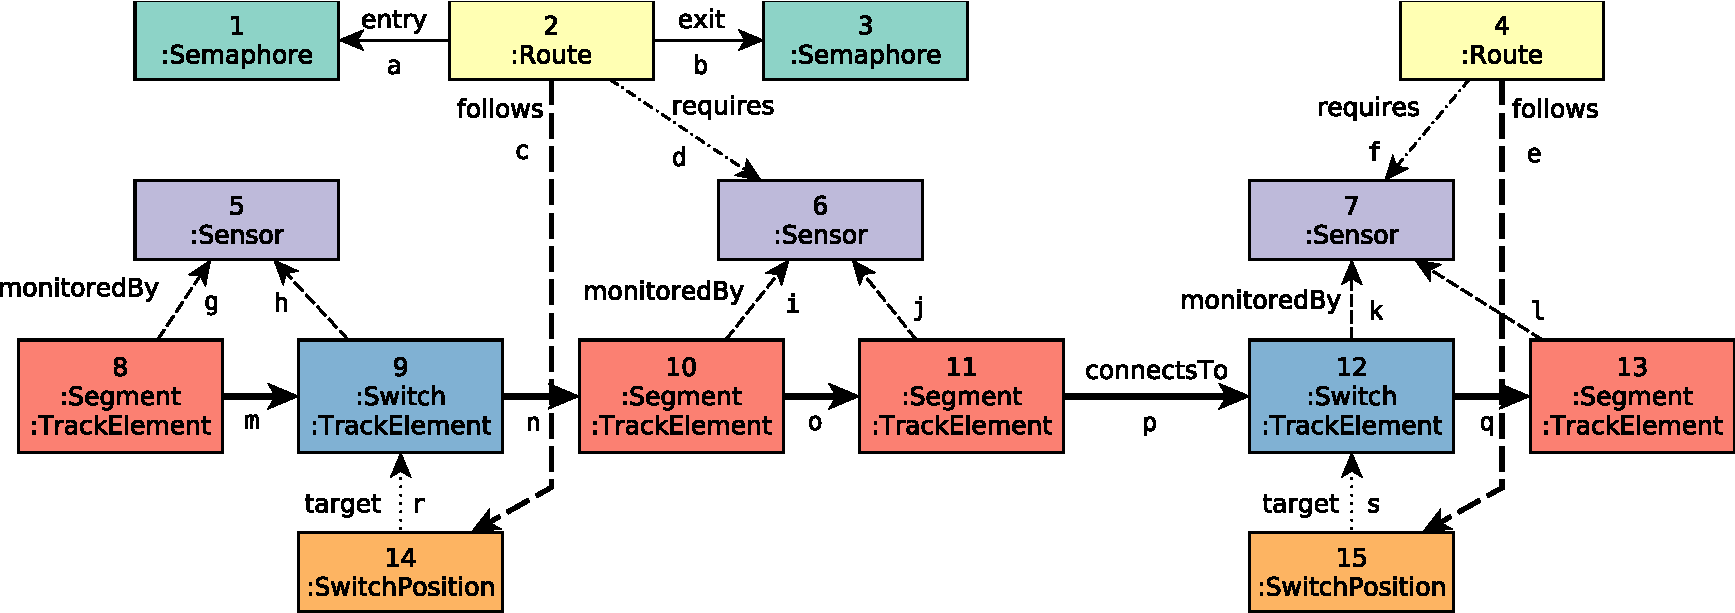
\includegraphics[scale=0.50]{trainbenchmark-instance-model}
	\caption{Example railway instance model as a labeled graph}
	\label{fig:trainbenchmark-instance-model}
\end{figure}

\section{Overview of Rete Networks}
\label{sec:rete}

\begin{figure}
	\centering
	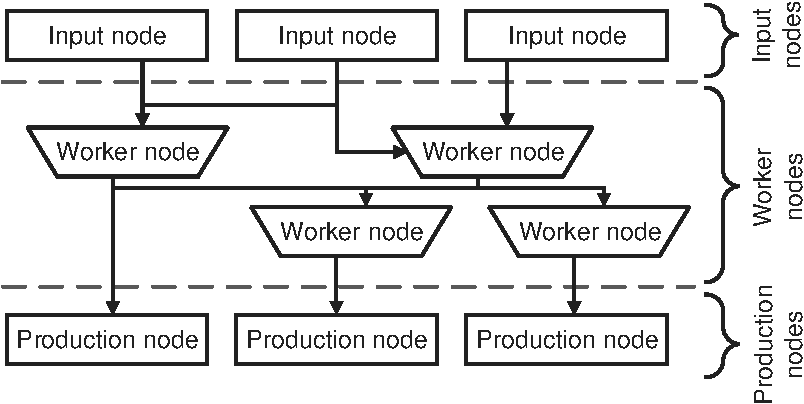
\includegraphics[width=8.5cm]{rete/rete}
	\caption{The structure of the Rete propagation network.}
	\label{fig:rete/rete}
\end{figure}

\todo{Draw a Rete network in tikz}

The Rete algorithm constructs a network of three types of nodes. Following \autoref{fig:rete/rete}, from bottom to top:

\begin{enumerate}
	\item \emph{Input nodes} are responsible for indexing the graph, \ie they store the appropriate tuples for vertices and edges in the graph. They are also responsible for sending \emph{change sets} as \emph{update messages} to worker nodes that are \emph{subscribed} to them.
	\item \emph{Worker nodes} perform a relational algebraic operation on their input and propagate the results to other worker nodes or production nodes. Some worker nodes are \emph{stateful}: they store partial query results in their memory to allow incremental reevaluation.
	Worker nodes have two types: \emph{unary nodes} have a single input slot, \emph{binary nodes} have two input slots.
	\item \emph{Production nodes} are terminators that provide an interface for fetching the results.
\end{enumerate}

The Rete network operates as follows. First, the network computes the set of pattern matches in the graph. Then upon a change in the graph, the network is incrementally maintained by propagating \emph{update messages} (also known as \emph{deltas}, denoted with the $\Delta$ character). Adding new graph matches to the result set is expressed as \emph{positive update messages}, while removing matches results in \emph{negative update messages}.

%\section{Rete Nodes}

In the following, we discuss Rete nodes in detail. For unary and binary nodes, we formulate the \emph{maintenance operations}, which are performed upon receiving an update message. For these operations, we denote the output relation by $t$, the updated output relation by $t'$, and the propagated update message on the output by $\Delta t$. If the \emph{propagated update message} is a positive update, $t' = t \cup \Delta t$, if it is a negative update, $t' = t \setminus \Delta t$.

\section{Input Nodes}

%\fig{rete/input-node}{Graphical notation of an input node}{\retescale}

\emph{Input nodes} provide the relations for each label of the graph. For example, the input node for the $\mathsf{requires}$ edge label of example the graph (\autoref{fig:trainbenchmark-instance-model}) returns tuples that are currently in the $\mathit{requires}$ relation: $ \left\{ \tuple{2, d, 6}, \tuple{4, f, 7} \right\} $. This input node is also responsible for propagating changes to worker nodes in the network:

\begin{itemize}
	\item If a $\mathsf{requires}$ edge `t' is inserted from vertex 2 to 5, the input node sends a positive update message to its subscriber nodes with the change set $ \left\{ \tuple{2, t, 4} \right\} $.
	\item If the edge `d' between vertices 2 and 6 is deleted, the input node sends a negative update to its subscriber nodes with the change set $ \left\{ \tuple{2, d, 6} \right\} $.
\end{itemize}

The relations contained by input nodes can be defined with nullary operators (\autoref{sec:nullary-operators}): input nodes indexing vertices implement the \getverticestext operator, while input nodes indexing edges implement the \getedgestext operator.

\section{Unary Nodes}

%\fig{rete/unary-node}{Graphical notation of a unary node}{\retescale}

\emph{Unary nodes} have one input slot. They filter or transform the tuples of the parent node according to certain criteria. In the following, the relation representing the input tuples is denoted with $r$, the relation representing the output tuples is denoted with $t$, and the operator processing the input is denoted with $\alpha$:
\begin{align*}
t = \op{\alpha}{r}.
\end{align*}

\subsubsection{Maintenance}

In the following, we assume that the $\alpha$ operator is \emph{distributive} \wrt the union ($\union$) and set minus ($\setminus$) operators. If a unary node receives an update $\Delta r$, it performs the operation and computes the change set. For \emph{positive updates}, the result ($t'$) and the changeset ($\Delta t$) are:
\begin{align*}
	t'       & \equiv \op{\alpha}{r \union \Delta r} \\
			 & = \op{\alpha}{r} \union \op{\alpha}{\Delta r} \\
			 & = t \union \underbrace{\op{\alpha}{\Delta r}}_{\Delta t} \\
\end{align*}

Similarly, for \emph{negative updates}:
\begin{align*}
	t'       & \equiv \op{\alpha}{r \setminus \Delta r} \\
			 & = \op{\alpha}{r} \setminus \op{\alpha}{\Delta r} \\
			 & = t \setminus \underbrace{\op{\alpha}{\Delta r}}_{\Delta t}
\end{align*}

Unary nodes are often implemented as \emph{stateless} nodes, \ie they do not store the results of the previous executions. Instead, these results are cached in their subscribers, \eg indexers of \emph{binary nodes} (\autoref{sec:binary-nodes}) or \emph{production nodes} (\autoref{sec:production-node}).

As their name suggests, unary nodes implement unary relational algebraic operators (\autoref{sec:unary-operators}):

\begin{itemize}
	\item The \emph{projection node} performs a projection operation on the input relation.
	\item The \emph{selection node} performs a selection operation on the input relation.
	\item The \emph{all-different node} \ldots
	\item The \emph{grouping node} \ldots
	\item The \emph{unwind node} \ldots
	\item The \emph{top node} \ldots
\end{itemize}

As all operators are distributive \wrt the union and set minus operators \todo{are they? prove}, their results can be maintained by performing the operation for the change set $\Delta r$.

\section{Binary Nodes}
\label{sec:binary-nodes}

%\fig{rete/binary-node}{Graphical notation of a binary node}{\retescale}

\emph{Binary nodes} implement \emph{binary relational operators} (\autoref{sec:binary-operators}) and
have two input slots: the \emph{primary} ($p$) and the \emph{secondary} ($s$). Binary node implementations typically cache both their input relations in \emph{indexers}.

\subsection{Natural Join Node}

\subsubsection{Maintenance}

In the following, we define the maintenance operations for natural join nodes. If a natural join node receives a \emph{positive update} $\Delta p$ on its \emph{primary} input slot, the result ($t'$) and the change set ($ \Delta t$) are determined as follows:
\begin{align*}
	t'       & \equiv \left(p \cup \Delta p\right) \join s           \\
	         & = (p \join s) \union (\Delta p \join s) \\
	         & = t \union \underbrace{(\Delta p \join s)}_{\Delta t}
\end{align*}

If the node receives a \emph{positive update} $\Delta s$ on its \emph{secondary} input slot, the result ($t'$) and the change set ($ \Delta t$) are the following:
\begin{align*}
	t'       & \equiv p \join \left(s \cup \Delta s\right)           \\
	         & = (p \join s) \union (p \join \Delta s) \\
	         & = t \union \underbrace{(p \join \Delta s)}_{\Delta t}
\end{align*}

For \emph{negative updates}, the changeset is the same, but it is propagated as a \emph{negative update}. The result is $t' = t \setminus (\Delta p \join s)$ and $t' = t \setminus (p \join \Delta s)$, for updates messages on the primary and the secondary input slots, respectively.

\subsection{Antijoin Node}

\subsubsection{Maintenance}

As the antijoin operator is not commutative, handling update messages requires us to distinguish between the following cases:

\begin{itemize}
	\item Update on the primary slot.
	\begin{itemize}
		\item Positive update: send a \emph{positive update} for each incoming tuple for which there is no match on the secondary indexer.
		\begin{align*}
			t'       & \equiv \left(p \cup \Delta p\right) \antijoin s               \\
			         & = (p \antijoin s) \union (\Delta p \antijoin s) \\
			         & = t \union \underbrace{(\Delta p \antijoin s)}_{\Delta t}
		\end{align*}

		\item Negative update: send a \emph{negative update} with the following tuples:
		$$ \Delta t = \Delta p \antijoin s $$
	\end{itemize}

	\item Update on the secondary slot. This case is more difficult to handle, so we recall the definition of the antijoin operator from \autoref{sec:binary-operators} for relations $p$ and $s$:
	\begin{align*}
		t & \equiv p \antijoin s = p \setminus \left(p \join \pi_{P \cap S} (s)\right),
	\end{align*}




	%t & \equiv p \antijoin s \\
	%&= p \setminus \pi_{P} \left(p \join s\right),

	\begin{itemize}
		\item For positive updates, the result set can be expressed as:
		\begin{align*}
			t'       & \equiv p \antijoin \left(s \cup \Delta s\right) \\
			         & = p \setminus \left( p \join \pi_{P \cap S} \left(s \cup \Delta s\right) \right)
		\end{align*}

		Positive updates on the secondary indexer result in \emph{negative updates} on the result set, so that $t' = t \setminus \Delta t$, hence $\Delta t = t \setminus t'$.

		For sets $A, B \subseteq C$, the following equality holds: $(C \setminus A) \setminus (C \setminus B) = B \setminus A$.
		Applying this with $C = p$ and using the distributive property of the natural join operator, the change set can be determined as:
		\begin{align*}
		\Delta t = t \setminus t' & = \overbrace{\left[p \setminus \left(p \join \pi_{P \cap S} (s)\right)\right]}^{t} \setminus \overbrace{\left[p \setminus \left( p \join \pi_{P \cap S} \left(s \cup \Delta s\right) \right)\right]}^{t'} \\
		         & = \left( p \join \pi_{P \cap S} \left(s \cup \Delta s\right) \right) \setminus \left(p \join \pi_{P \cap S} (s)\right) \\
		         & = p \join \left(\pi_{P \cap S} (s \cup \Delta s) \setminus \pi_{P \cap S} (s) \right) \\
		         & = p \join \left(\pi_{P \cap S} (s) \cup \pi_{P \cap S} (\Delta s) \setminus \pi_{P \cap S} (s) \right) \\
		         & = p \join \left(\pi_{P \cap S} (\Delta s) \setminus \pi_{P \cap S} (s) \right)
		\end{align*}

		\item For negative updates, the result set can be expressed as:
		\begin{align*}
		t' & \equiv p \antijoin \left(s \setminus \Delta s\right) \\
		   & = p \setminus \left(p \join \pi_{P \cap S} \left(s \setminus \Delta s\right)\right),
		\end{align*}

		Negative updates may result in \emph{positive updates} on the result set. Since $t' = t \union \Delta t$, we can define $\Delta t = t' \setminus t$:
		\begin{align*}
		\Delta t = t' \setminus t & = \overbrace{\left[p \setminus \left( p \join \pi_{P \cap S} \left(s \setminus \Delta s\right) \right)\right]}^{t'} \setminus \overbrace{\left[p \setminus \left(p \join \pi_{P \cap S} (s)\right)\right]}^{t} \\
		         & = \underbrace{\left(p \join \pi_{P \cap S} (s)\right)}_{x} \setminus \underbrace{\left( p \join \pi_{P \cap S} \left(s \setminus \Delta s\right) \right)}_{y}
		\end{align*}
		Although this change set may seem difficult to calculate, we point out that both $x$ and $y$ can be maintained incrementally. Furthermore, they only grow linearly in the size of $p$, as the join operator does not introduce new attributes, hence it can only reduce the number of elements in the relation.
	\end{itemize}
\end{itemize}


\subsection{Left Outer Join Node}

\begin{align*}
	t' & \equiv p \leftouterjoinop s
\end{align*}

\todo{TODO: define maintenance operators}

\subsection{Union Node}

\begin{align*}
	t' & \equiv (p \union \Delta p) \union s \\
	   & = (p \union s) \union \Delta p \\
	   & = t \union \underbrace{\Delta p}_{\Delta t}
\end{align*}

As the union operator is commutative, for updates on the secondary input, the rules are the same, but $p$ and $s$ are changed and $\Delta p$ is renamed to $\Delta s$.

\section{Production Nodes}
\label{sec:production-node}

\emph{Production nodes} are terminators that provide an interface for fetching results of a query (the match set) and also propagate the changes introduced by the latest update message.\footnote{In popular Rete implementations, clients are usually subscribed to the production nodes and notified about the changes in the result set.}

\subsubsection{Maintenance}

The change set is defined as:
$$\Delta t \equiv \bigunion_{i=1}^{n} \Delta r_i,$$

where $\Delta r_1, \Delta r_2, \ldots, \Delta r_n$ are the update messages triggered by the last change.
%For positive update messages, $t' = t \union \Delta t,$ while for negative update messages $t' = t \setminus \Delta t.$
